\subsection{Организационно-экономическая характеристика ООО <<Агрофирма Острожка>>}

\begin{figure}[hb]
	\centering
	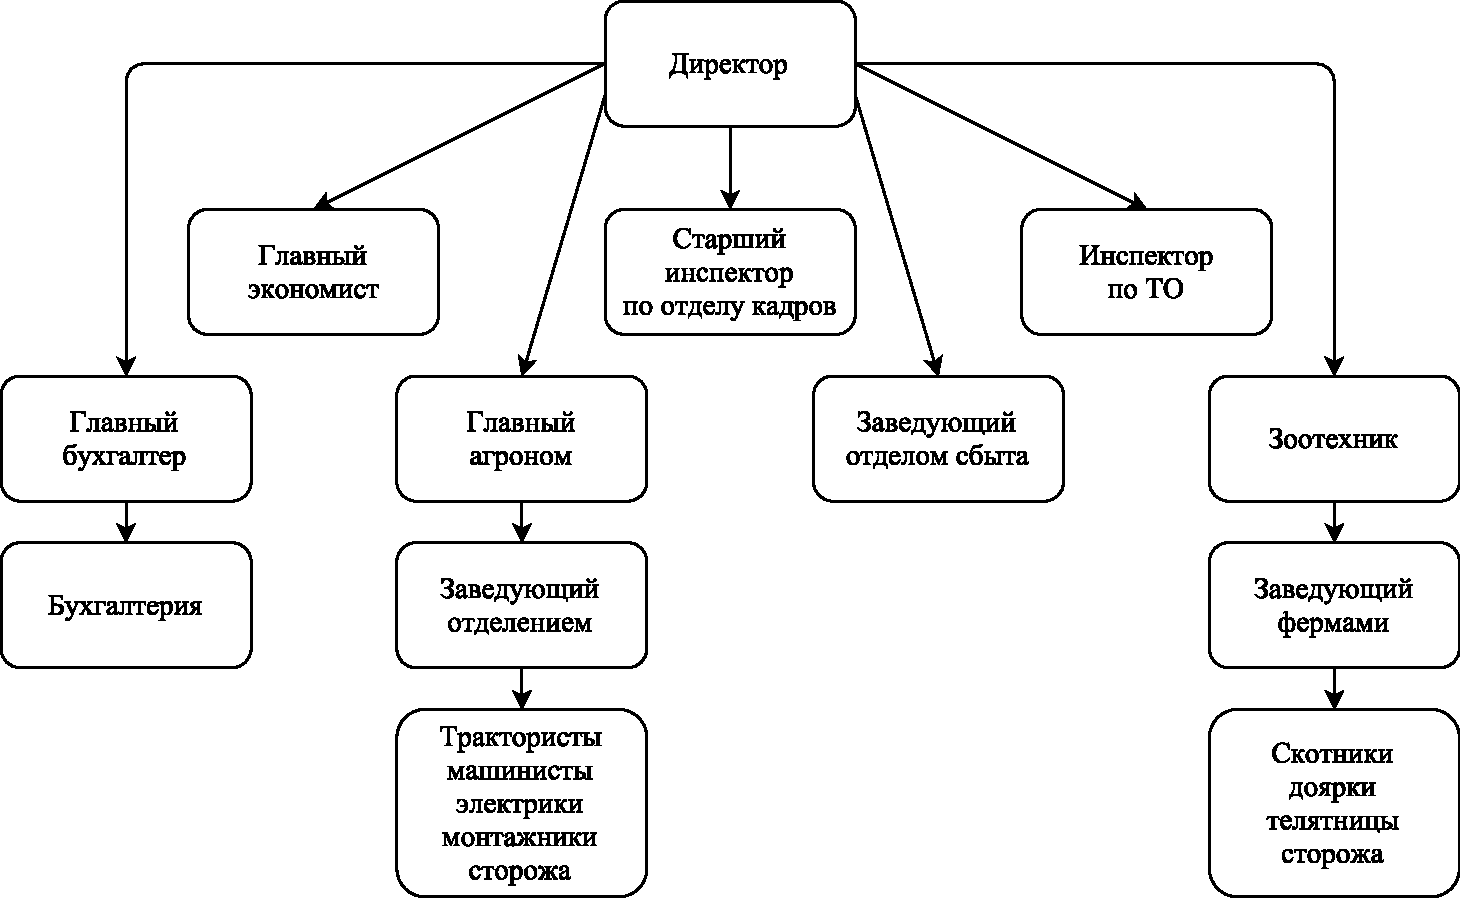
\includegraphics[width=0.8\linewidth]{fig2}
	\caption{Структура управления ООО «Агрофирма Острожка» в 2017 году}
	\label{fig:fig1}
\end{figure}

Общество с ограниченной ответственностью «Агрофирма Острожка», создано в целях получения прибыли от предпринимательской деятельности в порядке преобразования производственного сельскохозяйственного кооператива «Острожка», является его правопреемником и осуществляет свою деятельность в соответствии с Гражданским кодексом Российской Федерации, Федеральным законом Российской Федерации «Об обществах с ограниченной ответственностью», действующим российским законодательством.

Место нахождения Общества: 618103, Пермский край, Оханский район с. Острожка ул. Советская, д.42,

Организация зарегистрирована 31 декабря 2014 г.

Руководитель организации: директор Таскаев Николай Сергеевич.

Общество в настоящее время является сельхозтоваропроизвоителем и применяет специальный режим налогообложения – единый сельскохозяйственный налог (ЕСХН).

Основным видом деятельности является «Разведение молочного крупного рогатого скота, производство сырого молока», зарегистрировано 19 дополнительных видов деятельности. Организации ООО <<Агрофирма Острожка>> присвоены ИНН 5947000343, ОГРН 1145958090475, ОКПО 26591889.

Высшим органом управления ООО «Агрофирма Острожка» является общее собрание учредителей.

Текущей деятельностью организации руководит директор.

В ООО «Агрофирма Острожка» применяется линейно-функциональная (штабная) структура управления, которая обеспечивает проведение единоначалия и создает предпосылки для квалифицированного руководства соответствующими подразделениями.

\begin{table}[!ht]
	\small
	\centering
	\caption{Динамика состава трудовых ресурсов в 2014--2016 гг.}
	\label{dynamictrud}
	\setlength{\extrarowheight}{1mm}
	\begin{tabularx}{\textwidth}{|p{3.85cm}|K{1cm}|K{1cm}|K{1cm}|K{1cm}|K{1cm}|K{1cm}|K{1.6cm}|K{1.6cm}|}
		\hline
		\multirow{3}{3cm}{Категории персонала}   & \multicolumn{6}{c|}{Год}                                                                                                                                        & \multicolumn{2}{c|}{Изменение}                                                  \\ \cline{2-9} 
		& \multicolumn{2}{c|}{2014 г.} & \multicolumn{2}{c|}{2015 г.} & \multicolumn{2}{c|}{2016 г.} & 2015 г. к 2014 г. & 2016 г. к 2015 г. \\ \cline{2-9} 
		& Чел. & \% & Чел. & \% & Чел. & \% & Чел.& Чел. \\ \hline
		Среднегодовая численность, всего, чел. & 152                       & 100                     & 142                       & 100                     & 129                       & 100                     & -10                                    & -13                                    \\ \hline
		В т.ч по основной деятельности         & 147                       & 96,3                    & 139                       & 97,9                    & 128                       & 99,2                    & -8                                     & -11                                    \\ \hline
		Из них:                                &                           &                         &                           &                         &                           &                         &                                        &                                        \\
		руководители                           & 14                        & 9,2                     & 12                        & 8,5                     & 12                        & 9,3                     & -2                                     & -                                      \\ \hline
		специалисты                            & 8                         & 5,3                     & 8                         & 5,6                     & 6                         & 4,6                     & -                                      & -2                                     \\ \hline
		рабочие                                & 125                       & 82,2                    & 119                       & 83,8                    & 110                       & 85,3                    & -6                                     & -9                                     \\ \hline
		прочие                                 & 5                         & 3,3                     & 3                         & 2,1                     & 1                         & 0,8                     & -2                                     & -2                                     \\ \hline
	\end{tabularx}
\end{table}

Структура управления создается самим предприятием, утверждается руководителем предприятия, и периодически совершенствуется в связи с изменением факторов, на нее влияющих.
На рисунке \ref{fig:fig1} представлена структура управления ООО «Агрофирма Острожка».





По данным таблицы \ref{dynamictrud}, трудовые ресурсы Общества, в основном, представлены четырьмя категориями работников. Подавляющее число сотрудников относится к категории «рабочие», что обусловлено спецификой деятельности сельскохозяйственного предприятия, и их доля на протяжении рассматриваемого периода имеет тенденцию к увеличению (с 82,2\% до 85,3\%). В то же время, доля руководителей и специалистов в разрезе отчётных периодов остаётся примерно той же (в сумме порядка 14\%).

Что касается динамики абсолютных показателей численности работников ООО «Агрофирма Острожка», следует отметить, что она имеет устойчивую тенденцию к снижению. За анализируемый период штат работников сельхозпроизводства сократился на 19 человек, в том числе  рабочих на 15 человек.









